\begin{frame}{Performance Results}
\begin{columns}[T] 
        \begin{column}{0.32\textwidth}
            \centering
            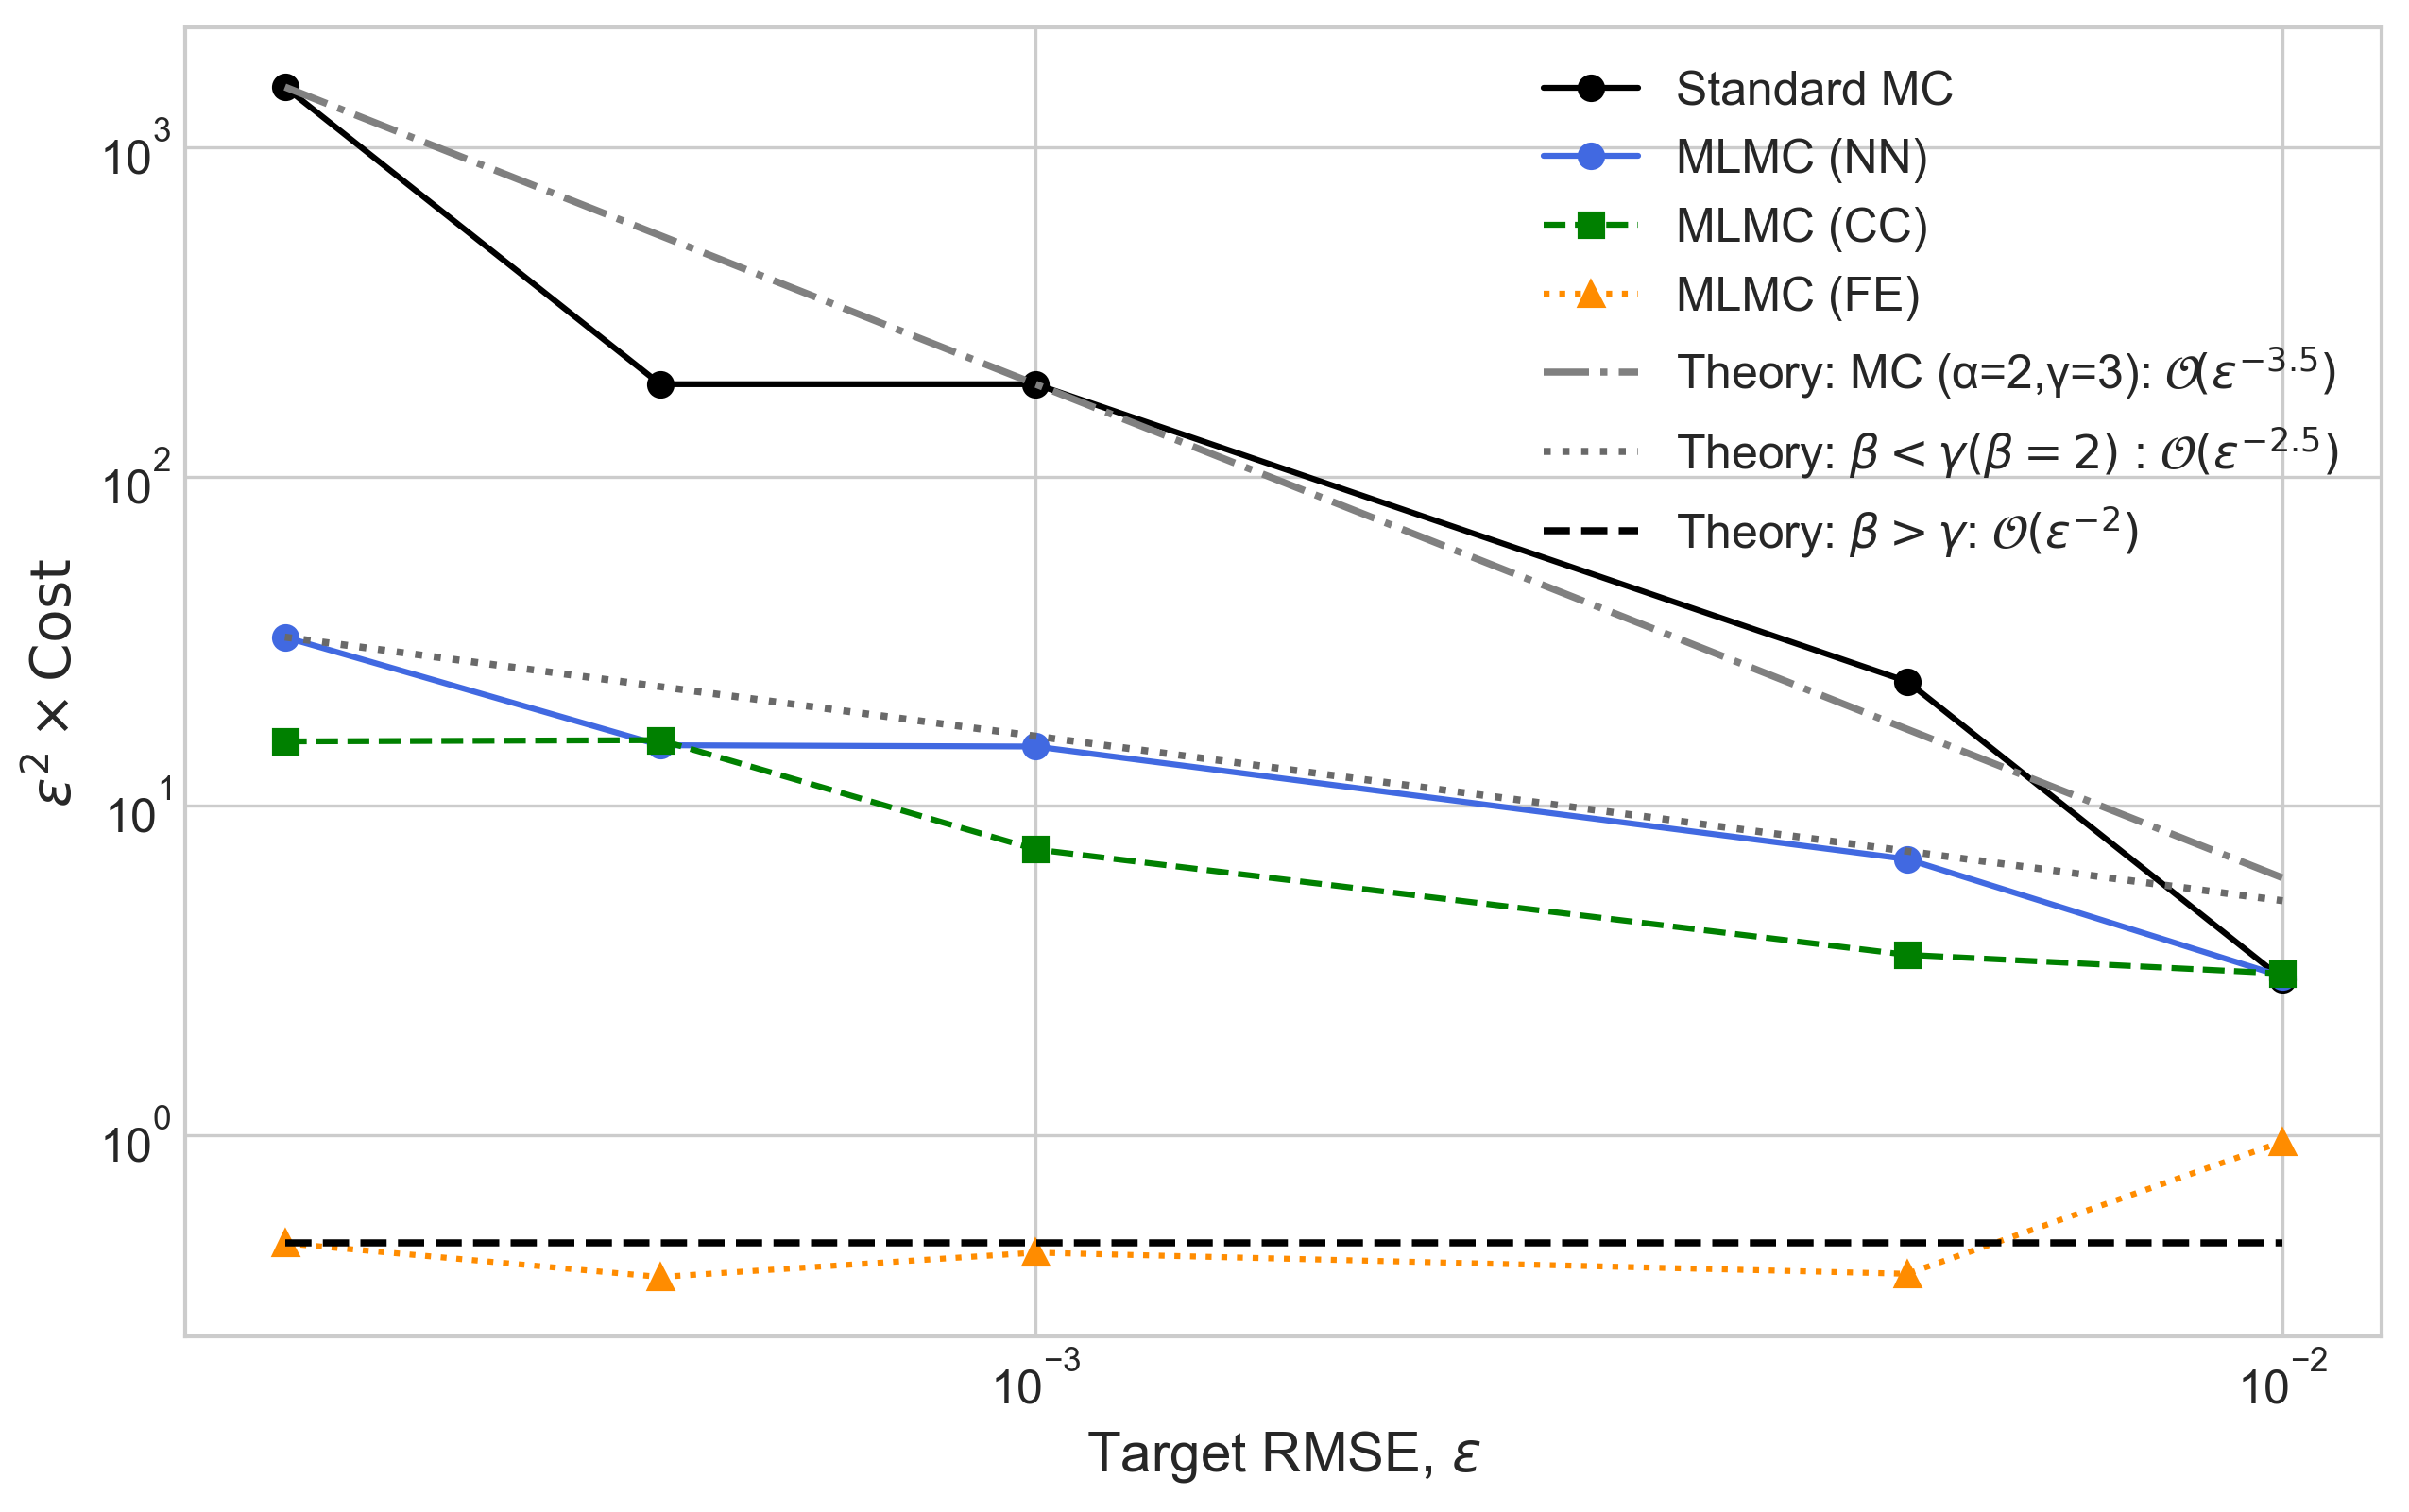
\includegraphics[height=2.7cm]{presentation_graphics/she_sq_amp_costs.png}
            {\scriptsize SHE - Squared Amplitude}
            \begin{itemize}\tiny
                \item FE coupling: optimal scaling $\mathcal{O}\left(\varepsilon^{-2}\right)$.
                \item NN and CC: both suboptimal  - $\mathcal{O}(\varepsilon^{-2-(\gamma-\beta) / \alpha})$.
            \end{itemize}
        \end{column}

        \begin{column}{0.32\textwidth}
            \centering
            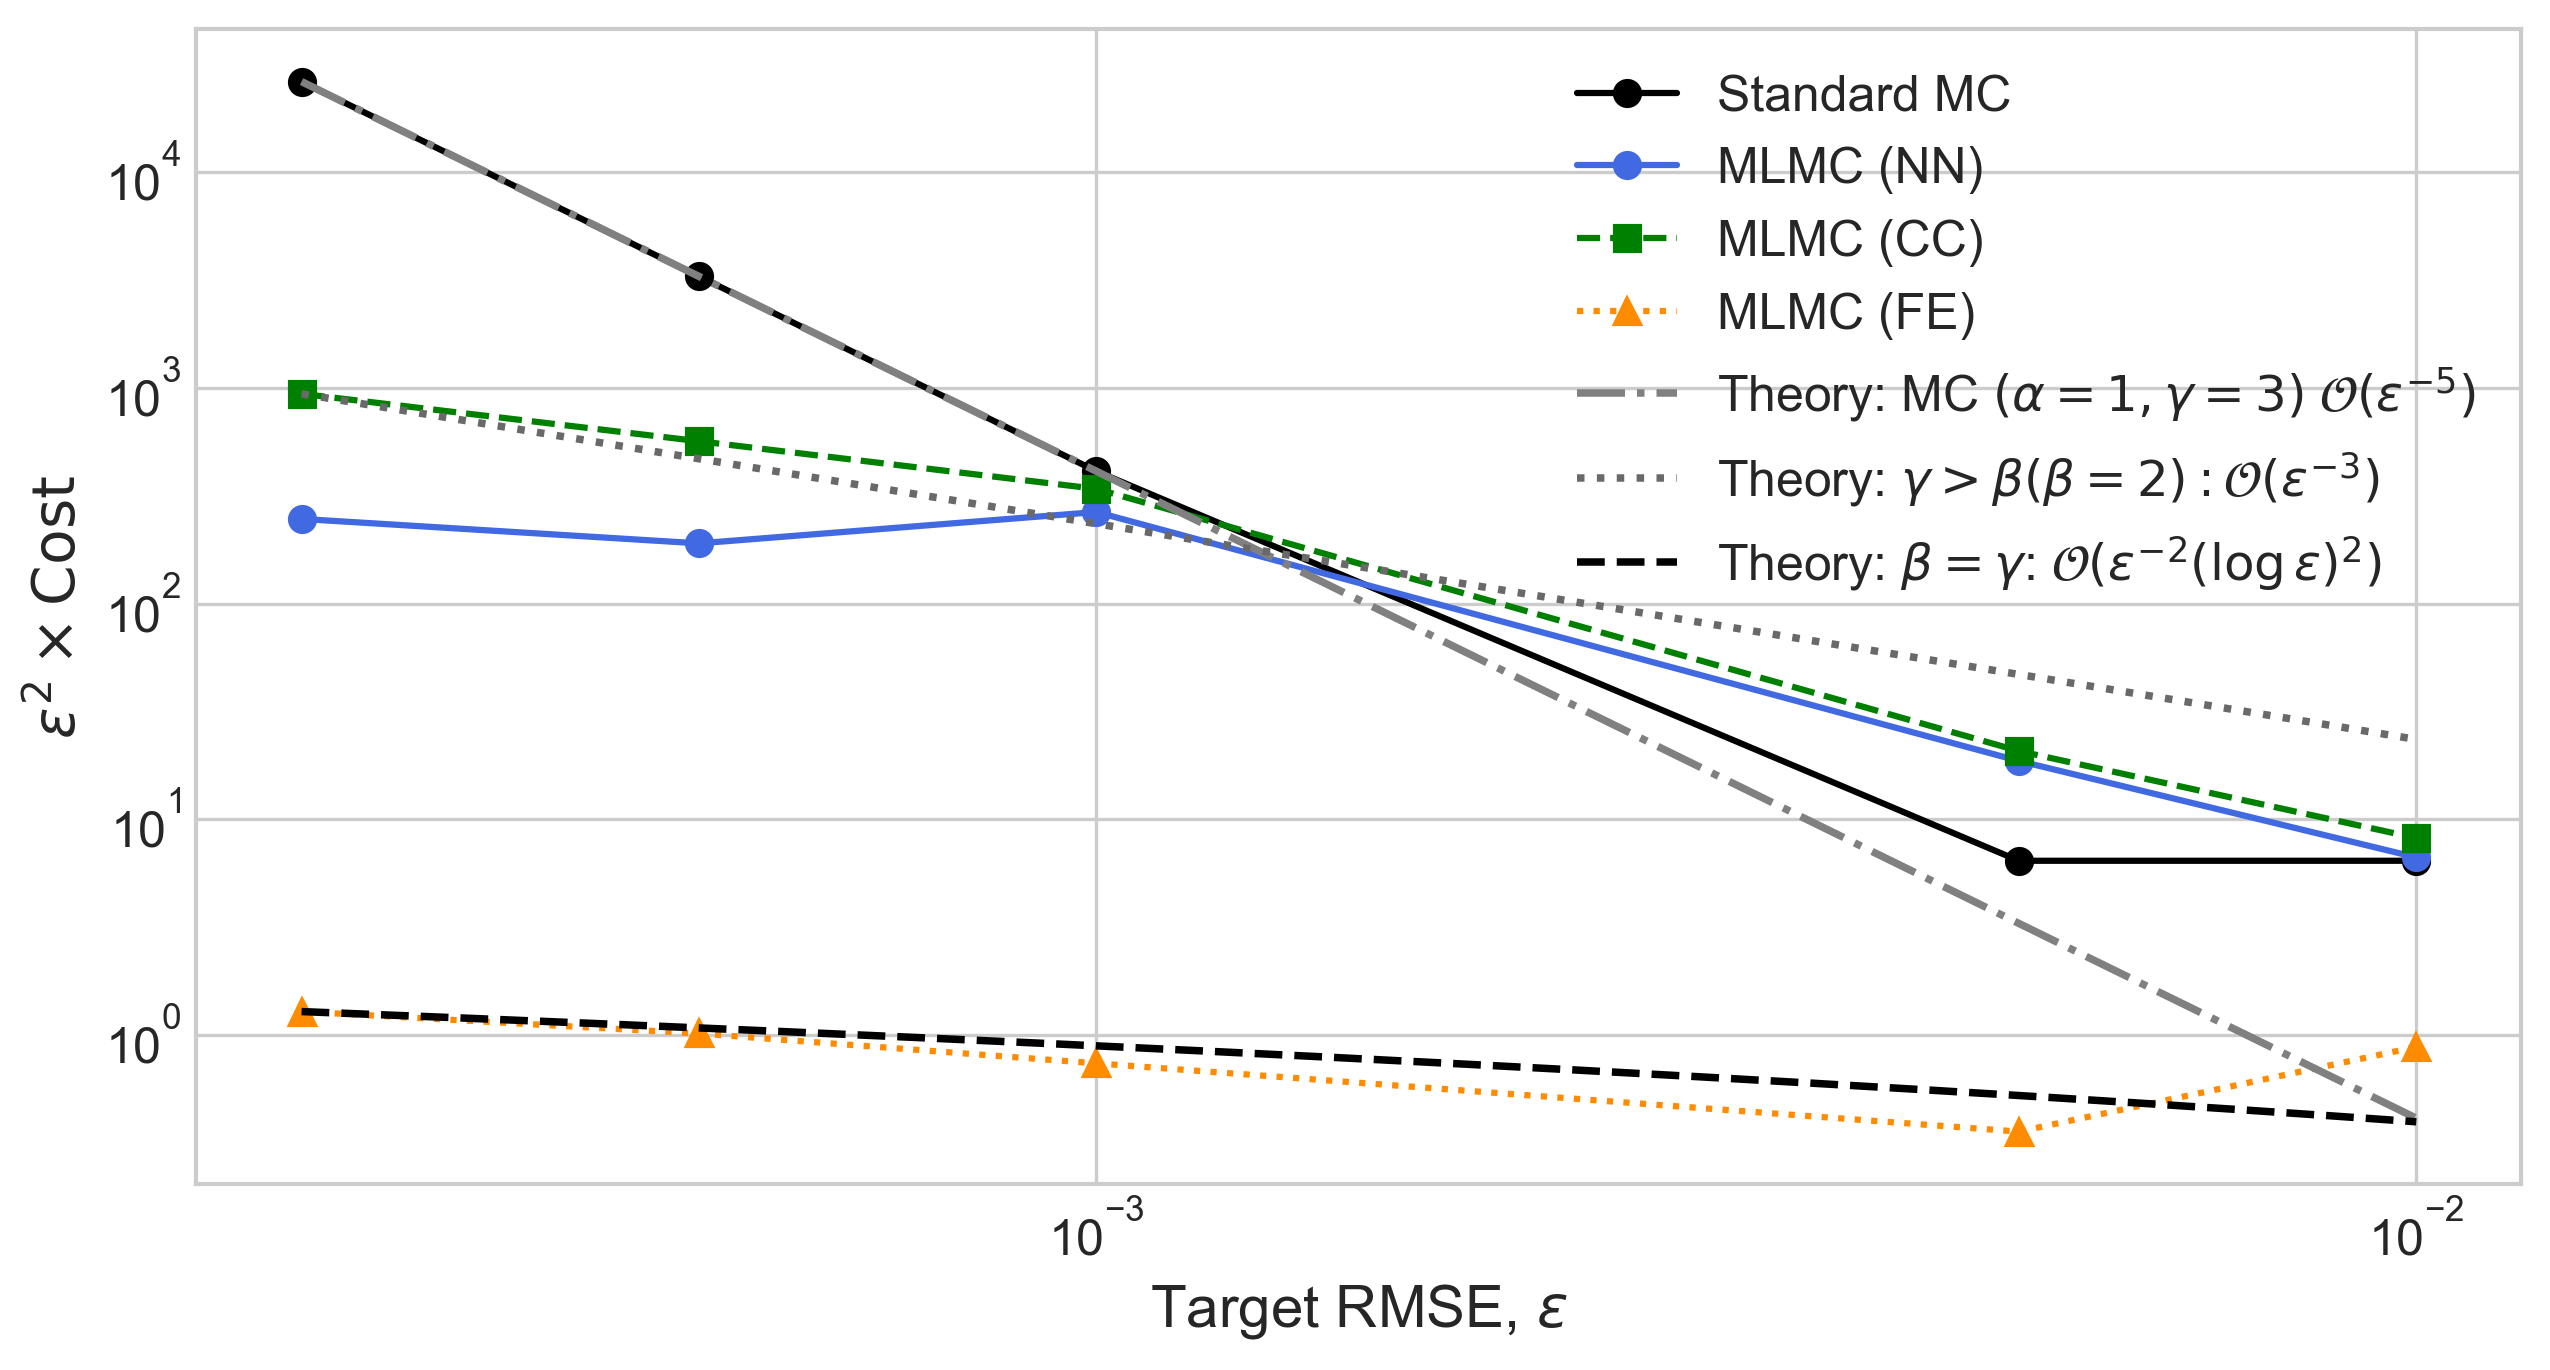
\includegraphics[height=2.7cm]{presentation_graphics/she_costs_energy.png}
            {\scriptsize SHE - Energy}
            \begin{itemize}\tiny
                \item FE coupling: near-optimal $\mathcal{O}\left(\varepsilon^{-2}(\log \varepsilon)^2\right)$.
                \item NN and CC: both suboptimal $\mathcal{O}(\varepsilon^{-2-(\gamma-\beta) / \alpha})$.
            \end{itemize}
        \end{column}

        \begin{column}{0.32\textwidth}
            \centering
            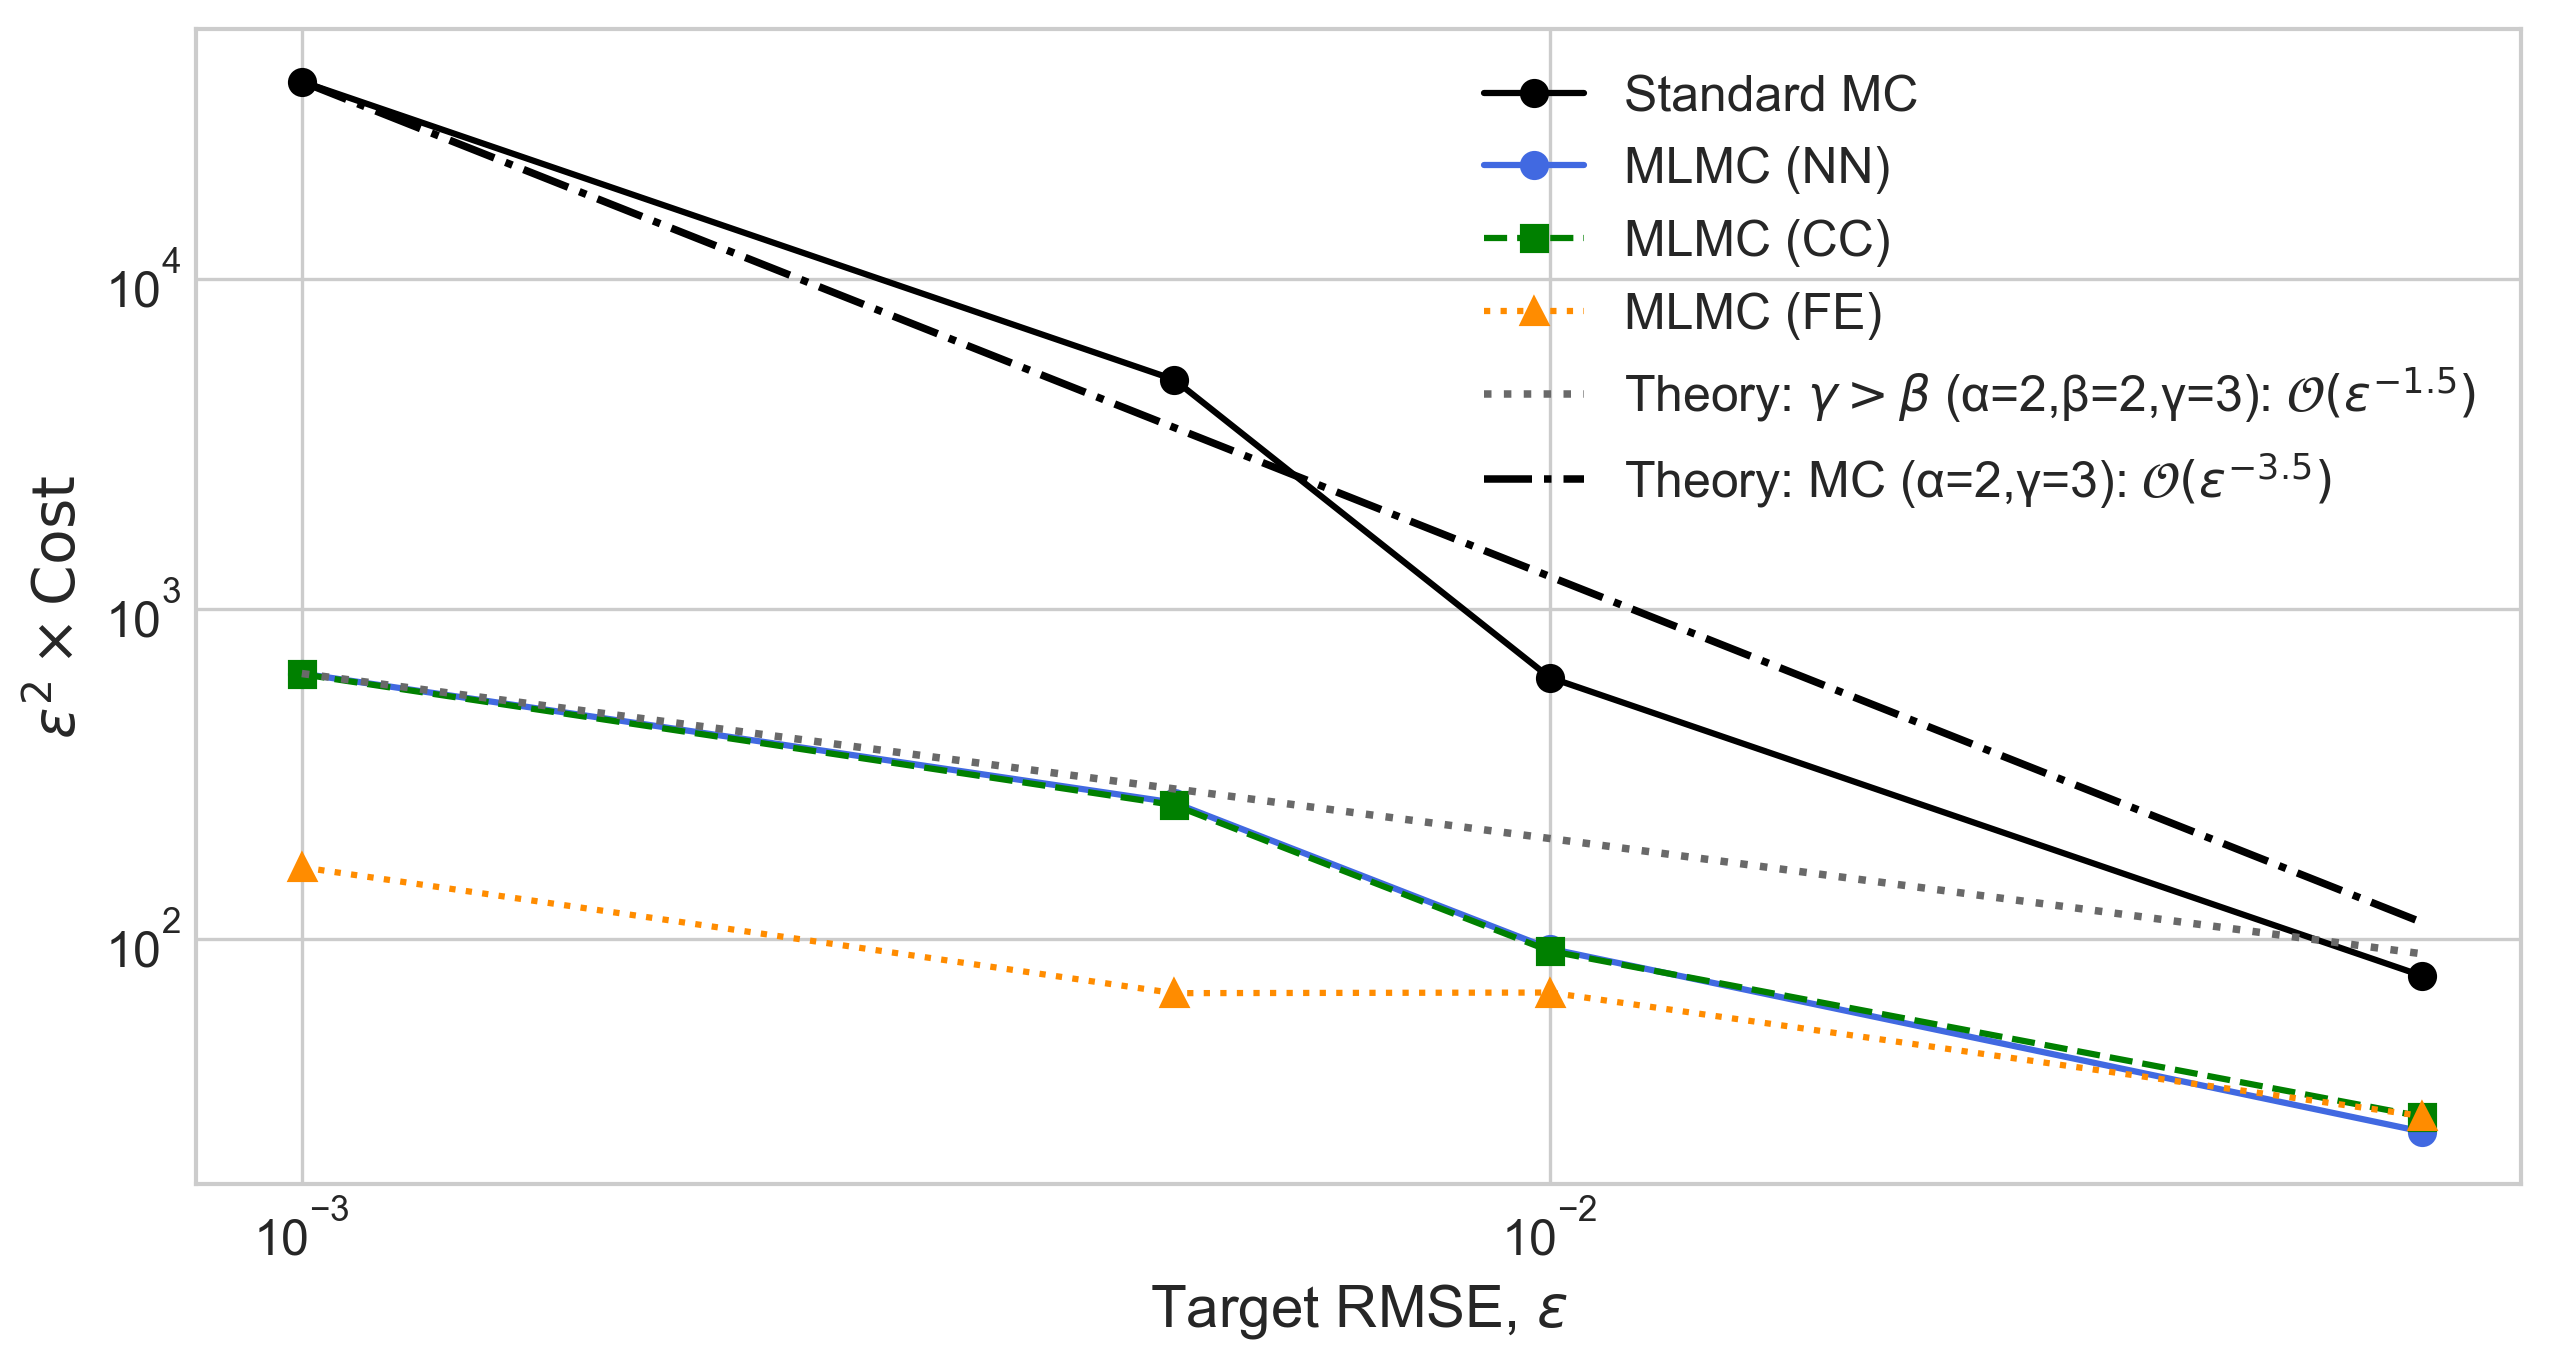
\includegraphics[height=2.7cm]{presentation_graphics/dk_costs.png}
            {\scriptsize DK - Mean Fluctuations}
            \begin{itemize}\tiny
                \item FE, NN and CC: equivalent scaling $\mathcal{O}(\varepsilon^{-2-(\gamma - \beta) / \alpha})$.
            \end{itemize}
        \end{column}
    \end{columns}
\end{frame}
